\documentclass[journal]{vgtc}                % final (journal style)
%\documentclass[review,journal]{vgtc}         % review (journal style)
%\documentclass[widereview]{vgtc}             % wide-spaced review
%\documentclass[preprint,journal]{vgtc}       % preprint (journal style)

%% Uncomment one of the lines above depending on where your paper is
%% in the conference process. ``review'' and ``widereview'' are for review
%% submission, ``preprint'' is for pre-publication, and the final version
%% doesn't use a specific qualifier.

%% These few lines make a distinction between latex and pdflatex calls and they
%% bring in essential packages for graphics and font handling.
%% Note that due to the \DeclareGraphicsExtensions{} call it is no longer necessary
%% to provide the the path and extension of a graphics file:
%% 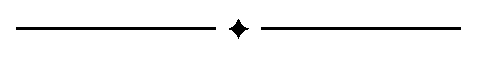
\includegraphics{diamondrule} is completely sufficient.
%%
\ifpdf%                                % if we use pdflatex
  \pdfoutput=1\relax                   % create PDFs from pdfLaTeX
  \pdfcompresslevel=9                  % PDF Compression
  \pdfoptionpdfminorversion=7          % create PDF 1.7
  \ExecuteOptions{pdftex}
  \usepackage{graphicx}                % allow us to embed graphics files
  \DeclareGraphicsExtensions{.pdf,.png,.jpg,.jpeg} % for pdflatex we expect .pdf, .png, or .jpg files
\else%                                 % else we use pure latex
  \ExecuteOptions{dvips}
  \usepackage{graphicx}                % allow us to embed graphics files
  \DeclareGraphicsExtensions{.eps}     % for pure latex we expect eps files
\fi%

%% it is recomended to use ``\autoref{sec:bla}'' instead of ``Fig.~\ref{sec:bla}''
\graphicspath{{figures/}{pictures/}{images/}{./}} % where to search for the images

\usepackage{microtype}                 % use micro-typography (slightly more compact, better to read)
\PassOptionsToPackage{warn}{textcomp}  % to address font issues with \textrightarrow
\usepackage{textcomp}                  % use better special symbols
\usepackage{mathptmx}                  % use matching math font
\usepackage{times}                     % we use Times as the main font
\renewcommand*\ttdefault{txtt}         % a nicer typewriter font
\usepackage{cite}

%% If you are submitting a paper to a conference for review with a double
%% blind reviewing process, please replace the value ``0'' below with your
%% OnlineID. Otherwise, you may safely leave it at ``0''.
\onlineid{0}

%% declare the category of your paper, only shown in review mode
\vgtccategory{Research}

%% Paper title.
\title{Coursim: A Tool For Detecting Course Similarity}

%% This is how authors are specified in the journal style

%% indicate IEEE Member or Student Member in form indicated below
\author{Yang Liu, Zhenge Zhao}
\authorfooter{
%% insert punctuation at end of each item
\item
 E-mail:[yangliu2014,your NetID2]@email.arizona.edu.
}

%other entries to be set up for journal
%\shortauthortitle{Firstauthor \MakeLowercase{\textit{et al.}}: Paper Title}

%% Abstract section.
\abstract{

CHANGE ME: Abstract goes here. It should briefly explain the problem, the big
picture of what was done to solve it, and the highlights of the results.

} % end of abstract

%% Keywords that describe your work. Will show as 'Index Terms' in journal
%% please capitalize first letter and insert punctuation after last keyword
%\keywords{Radiosity, global illumination, constant time}

%% ACM Computing Classification System (CCS). 
%% See <http://www.acm.org/class/1998/> for details.
%% The ``\CCScat'' command takes four arguments.

\CCScatlist{CHANGE ME:
 \CCScat{K.6.1}{Management of Computing and Information Systems}%
{Project and People Management}{Life Cycle};
 \CCScat{K.7.m}{The Computing Profession}{Miscellaneous}{Ethics}
}

% Comment below to remove teaser figure.
   \teaser{
   \centering
   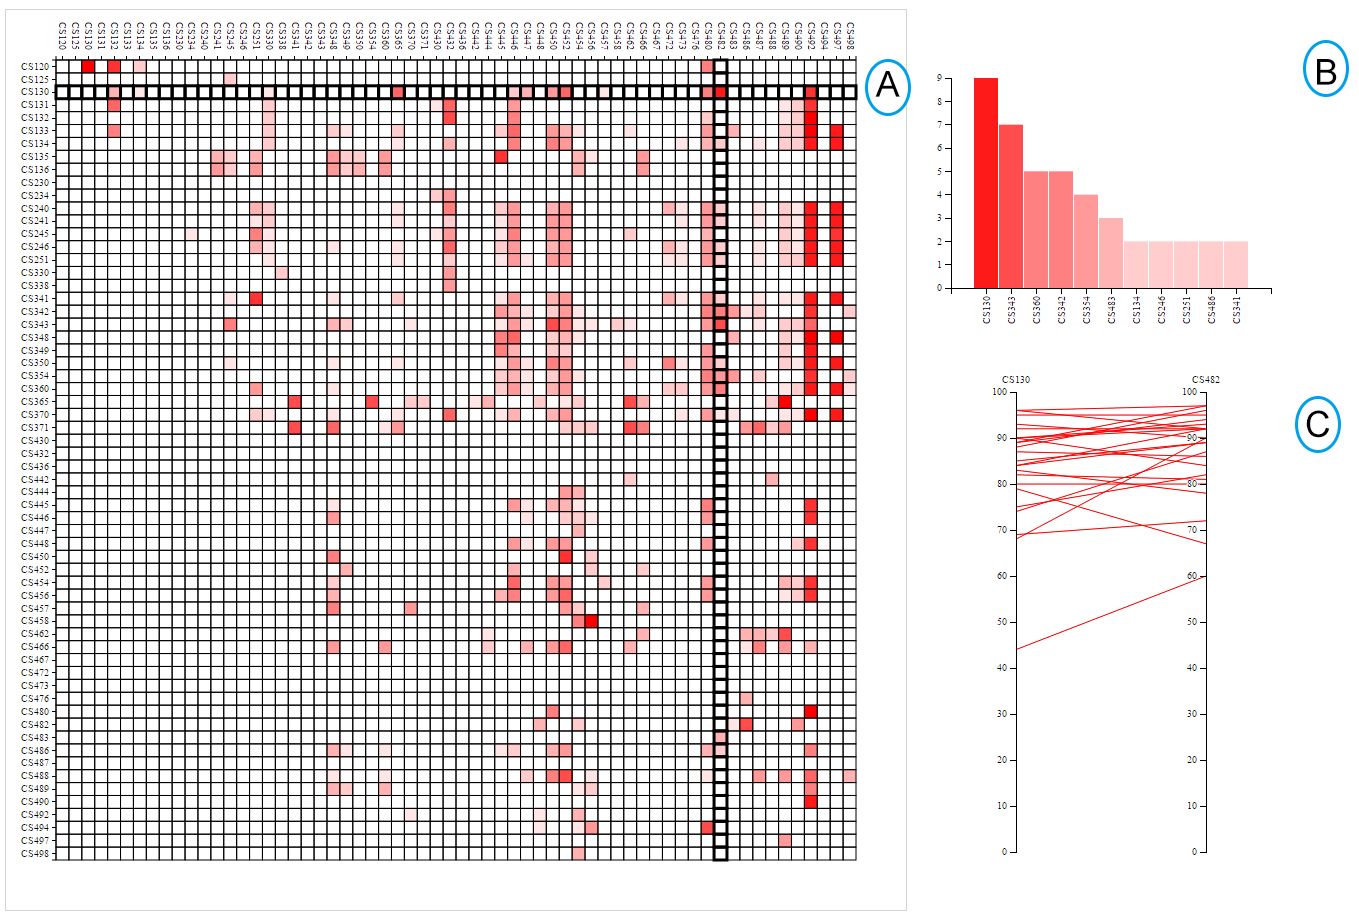
\includegraphics[width=16cm]{figs/perfvis}
   \caption{CHANGE ME: Some of you may want a big teaser figure.}
  }

%% Uncomment below to disable the manuscript note
%\renewcommand{\manuscriptnotetxt}{}

%% Copyright space is enabled by default as required by guidelines.
%% It is disabled by the 'review' option or via the following command:
% \nocopyrightspace

\vgtcinsertpkg

%%%%%%%%%%%%%%%%%%%%%%%%%%%%%%%%%%%%%%%%%%%%%%%%%%%%%%%%%%%%%%%%
%%%%%%%%%%%%%%%%%%%%%% START OF THE PAPER %%%%%%%%%%%%%%%%%%%%%%
%%%%%%%%%%%%%%%%%%%%%%%%%%%%%%%%%%%%%%%%%%%%%%%%%%%%%%%%%%%%%%%%%

\begin{document}

%% The ``\maketitle'' command must be the first command after the
%% ``\begin{document}'' command. It prepares and prints the title block.

%% the only exception to this rule is the \firstsection command


\firstsection{Introduction} % or "Motivation"

\maketitle

CHANGE ME: There is not a canonical way to organize the paper -- we've seen
different styles during this course. You may alter the order to match your
project. Depending on the project, you may want to split the sections into
multiple parts.

% Introduction and/or Motivation

Navigating the curriculum of educational institution, fulfilling prerequisite and choosing between course options has been a feature of the educational environment dating back to Plato’s inscription ``Let no one ignorant of geometry enter!'' inscribed at the entrance of his academy~\cite{anglin1994mathematics}. In efforts to remain competitive, course options at institutes of higher learning have exploded, often offering hundreds of course possibilities that satisfy their general education requirements~\cite{schwartz2009paradox}.

The real world scene is that coursework contents can be related, making one course as the prerequisite of the other will help students better learn knowledge and obtain better grades. Academic advisor, for example, deals with these issues a lot.

While some course dependencies have already been explicitly annotated in practice, more remain unclear and potential. In this work, we’d like to design a visualization view to group related courses in clusters based on student enrollment history, and another view to show correlations of two related courses based on the discrete grades of students who have enrolled both courses.

% Maybe you want to use a list:
The aims of this research are:
\begin{itemize}
  \item provide a tool to visualize coursework contents similarity based on student performance.
  \item explore different diagrams to handle the complexity of information
  \item study similarity metrics of two courses based on grade history of one student and multiple students.
\end{itemize}



\section{Background}
\label{sec:background}

Collaborative-filtering is a recommendation approach that uses similarity between users and the benefit they have received from items in the past to make recommendations. Three main approaches to collaborative filtering are memory-based, model-based and hybrid methods~\cite{Su:2009:SCF:1592474.1722966} . Memory-based approaches, specifically item-based recommender~\ref{fig:predict}, use an item-user rating matrix to compute pairwise similarities between items. In the contexts of courses, enrollment roster, previous courses students taken and grades course give, is a natural way to reason about course similarity.  

\begin{figure}[h]
 \centering % avoid the use of \begin{center}...\end{center} and use \centering instead (more compact)
 \includegraphics[width=\linewidth]{figs/predict}
 \caption{Typical student course grade table}
 \label{fig:predict}
\end{figure}

However the recommendation approaches are not appropriate for our problems, since they are used for making predictions which means, the approach is designed to fill in the missing values in the matrix. For our case, however, we want to figure out how two courses are correlated with each other. We don’t want to fill the matrix since it will blur the original data. What’ more, for each two courses we are only interested in the users who take both of them. Visualization is an effective and intuitive way to approach our goal.  

There’re many existing similarity measures to compare two entities. Well known metrics include Euclidean similarity, Jaccard(Tanimoto) similarity, Pearson Correlation Coefficient, cosine similarity and Log-likelihood similarity etc. Euclidean similarity measures the distance between courses grading vectors. Jaccard(Tanimoto) similarity is calculated by dividing the intersection of the sets by the union of those sets\cite{sandvig2005aacorn}. Cosine Similarity envision user’s ratings as points in space and measures the cosine of the angle between these lines drawn from origin to each point. The Log-likelihood similarity is a measure of how often items from 2 sets appear together versus how often they appear apart. Pearson Correlation Coefficient is a number between -1, 1. It measures the tendency of the rating vectors, paired one by one, and it’s typically used in early research papers. Its formula is given as $pearson-correlation(u,w) = \frac{cov(R_u,R_w)}{\sigma x \sigma y} $ where $cov$ stands for covariance and $\sigma x$ stands for standard deviation of $x$. We are interested in the strong positive correlation and the positive correlation as illustrated in~\ref{fig:psc}.

For our work, Euclidean similarity is not suitable because courses taken by more students will be added more distances. Jaccard(Tanimoto) similarity and Log-likelihood don’t count grades students get. We choose Pearson Correlation coefficient to indicate the similarity between two courses and based on that, we build our item-based recommender system and provide a way to measure the benefits between two courses.
\begin{figure}[h]
 \centering % avoid the use of \begin{center}...\end{center} and use \centering instead (more compact)
 \includegraphics[width=1.5in]{figs/psc_illustrated}
\caption{Pearson Correlation Illustrated}
 \label{fig:psc}
\end{figure}




\section{Related Work}
\label{sec:related}

Discuss the work related to your project -- include both visualization and
domain-specific references to the problem you're trying to solve. What do
these solutions do and in what ways are they insufficient for the problem you
are trying to solve. Do you build on any of these? If so, how?

For example, if my work has to do with Perfopticon~\cite{Moritz:2015:EuroVis}
or comparing request flows~\cite{Sambasivan:2013:InfoVis}, I would want to
cite them. ACM Digital Library makes it easy to get bib files for final.bib
and there are guides online for citing books~\cite{ware:2004:IVP},
theses~\cite{levoy:1989:DSV}, journal articles~\cite{Lorensen:1987:MCA}, and
conference proceedings~\cite{Nielson:1991:TAD}.



\section{Visual Design} % or "Research Plan"
\label{sec:vis}

Our ultimate goal, is to design a visualization tool for understanding courses interactions. Our target users are professors, students and academic advisors. We talk with graduate students and professors about what they need to summarize our tasks as below:
\begin{itemize}
	\item [T1] Overview of clusters of correlated courses
	\item [T2] For a specific course, find the courses which potentially benefit it and compare the importance of these courses
	\item [T3] For two selected courses, show details of student grades
\end{itemize}

We preprocess our original data and choose to use all the course records of computer science department for our implementations. We carefully select the visualization techniques which can be easily understood by users. Our system has three major view: the adjacency matrix, bar chart view and parallel coordinates view. In this section. We describe all the works we have done and the details of Coursim.%\~\ref{sec:background}

%\You may want to use figures to illustrate your point, such as
%\Figure~\ref{fig:sample}.

\subsection{Data Processing}
\label{sec:data}
Towards this end, we performed a pilot study using student data from a Canadian research university.  This data included all students who had taken a computer science course at that university between September 2001 and December 2011.

The data was in a comma-separated file made up of rows with 6 fields:  a unique, anonymized student identifier, the term (which could be Spring, Summer or Fall and the year), the subject ID (such as “CS” or “ENGL”), the course code (such as “101”), the percentile grade received and the student’s major.

The data needed to be preprocessed in preparation for the similarity calculation and the visualization.  A unique, sequential identifier was added to each line.  There was a variety of identifiers for problems students had in a course, such as “WD” indicating withdrawal, “DNR” indicating the final exam was not written.  These were replaced with 0 so that there would be a consistent, natural number domain for the grades.  Some of the course codes had an optional letter suffix, which would indicate if it was offered on-line or at another campus (for example).  These were removed and all courses with the same code were treated as the same value.

We removed courses and corresponding records which less than 10 students take in the data set on the basis that there was insufficient pairwise to measure the interactions between two courses. After these adjustments, the training set consisted of 37,392 students with data about 468,632 courses they took. There were 2,326 unique courses in the dataset.Specifically, for the computer science department, there are 61 courses, 2861 students, in total 38751 records.


\begin{figure}[h]
	\centering % avoid the use of \begin{center}...\end{center} and use \centering instead (more compact)
	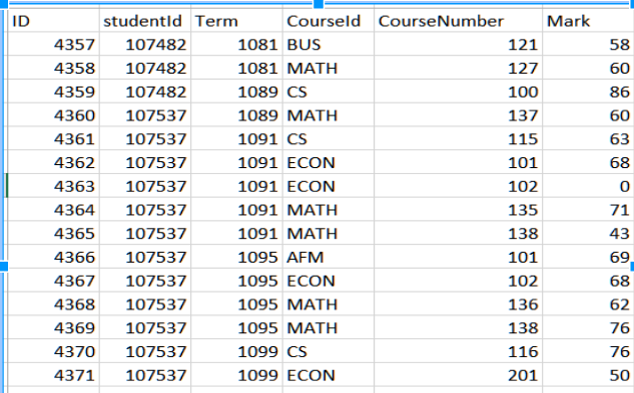
\includegraphics[width=\columnwidth]{figs/data} 
	\caption{Original data table}
	\label{fig:data}
\end{figure}

\subsection{Adjacency Matrix View}
\label{sec:matrix}
The Adjacency Matrix view enables users to grasp a global view of the all the courses. We use D3 library which contains the existing adjacency matrix template~\cite{Bostock:2011:DDD:2068462.2068631}. Each grid in the matrix represents the potential benefits the column course may get from the row course. Each row shows that, for a specific course, all the courses it may have a positive influence on. Each column depicts that, for a chosen course, all the courses which may benefit it. We build a mouse over in this view, when the users move their mouse on the grid, the column and the row associated with that gird chosen will be highlighted with a bold border which will make it easier to obverse the column and the row. The view also consists a zoomable and navigation feature which can be used to filter the uninterested data based on the demand. 

Adjacency Matrix view can clearly show the every possible connection between each pair of courses. Compared to node-link diagram or dagre layout~\cite{Bostock:2011:DDD:2068462.2068631}, it has obvious advantages in terms of recognition and orientation. When the size of the data get big, the force-directed node link diagram or dagre layout will include a lot of cross edges and become messy. It is hard for users to localize the actual pair of courses they want, and identify the actual relations between them. But adjacency matrix can always navigate users to the right pair of data and is easy for users to explore the data set and find interesting patterns. 

The color scale ranging from white to dark red indicates the similarity between each pair of courses. White grids mean either there are less than 10 students or the influence the one course has on the later course is negative. We talk about how we calculate the similarities measurement in the next section.
\begin{figure}[h]
	\centering % avoid the use of \begin{center}...\end{center} and use \centering instead (more compact)
	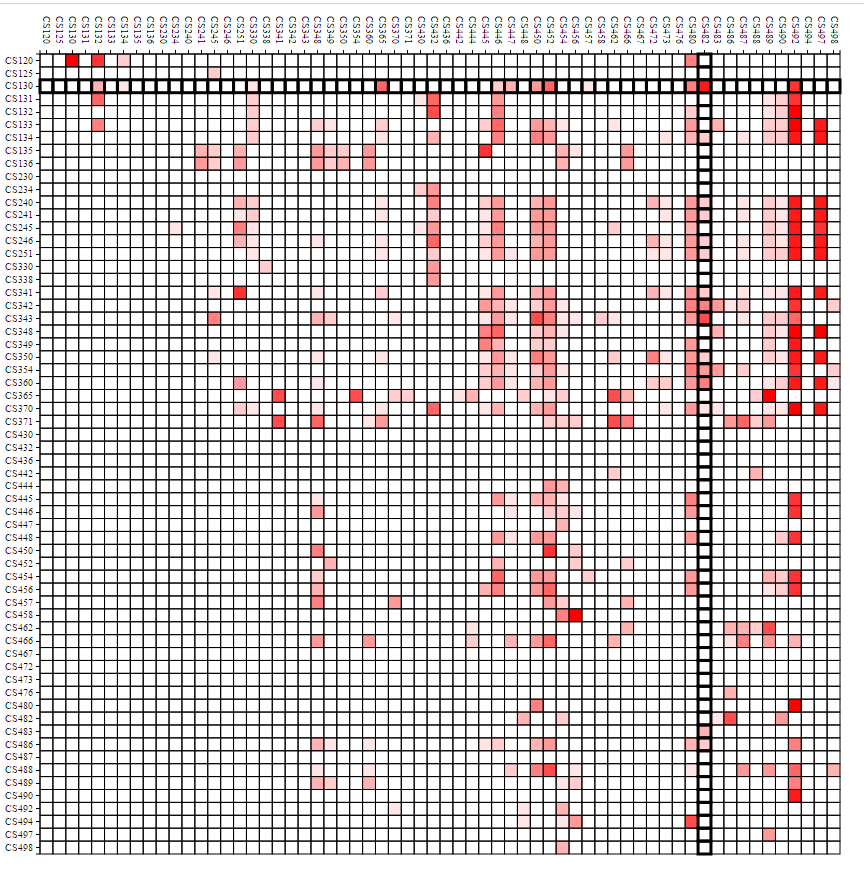
\includegraphics[width=\columnwidth]{figs/matrix} 
	\caption{Adjacency Matrix View}
	\label{fig:sample}
\end{figure}

\subsection{Benefits Measurement}
\label{sec:benefits}
In order to demonstrate the benefits a course(Pre1) may give to another(Course1), we want to build a measurement way based on students’ performance in both of the courses. The intuition is that if a student gets high scores in Pre1 and in the future semesters, they also get a high score in Course1, which may indicate the benefits between Pre1 and Course1. On the contrary, if the high score in Pre1 ends up with bad performance in Course1, the benefits may be few. Pearson-correlation seams a considerable method. But it turns out that it is not suitable in our case. The problem is that if for Pre1 and Course1, we extract the grades of the students who have taken both two courses in sequence and put them into two vectors. The results we get are not convincing. There are a few problems when applying Pearson-correlation. The first is that a lot of students’ performance is consistent. A student who can get high scores in one course will also achieve good scores in later courses. This makes the Pearson-correlation for each course very similar (around 0.7), which is hard to identify the benefits. Another problem is, the distribution of scores for different courses are also different. In some courses, 80 points may have been the one of best performance among all the students. The actual points depend on different professors and the different courses contain diverse standards.

In order to avoid the two problems mentioned above, we introduce a new benefit measurement based on recommender system. The motivation is that if a student(Jack) whose overall performance is not that good gets higher score in Course1 after taking Pre1 than the students whose overall performance are similar to Jack but without taking Pre1, we say Pre1 may be a benefit for course A.  We choose Collaborative Filtering which can predict a student’s grade on one course based on the similarity to other students. More specifically, we choose item-based recommender which is more efficient than the user-based recommenders since we have much fewer courses than the number of students.  To measure the benefit Pre1 may bring to Course1, we do as follows:
\begin{itemize}
	\item Step 1: For each course pair (in order, for example, Pre1, Course1) taken by more than 10 students, remove the actual grades of Course1 of those students and take the rest of the records of the training data. 
	\item Step 2 : Running an Item-based recommender using Pearson Correlation to predict the grades the students will get for Course1.
	\item Step 3: Calculating the average of the differences between the actual and predicted grades and take that as the similarity measurement.
\end{itemize}
\begin{figure}[h]
	\centering % avoid the use of \begin{center}...\end{center} and use \centering instead (more compact)
	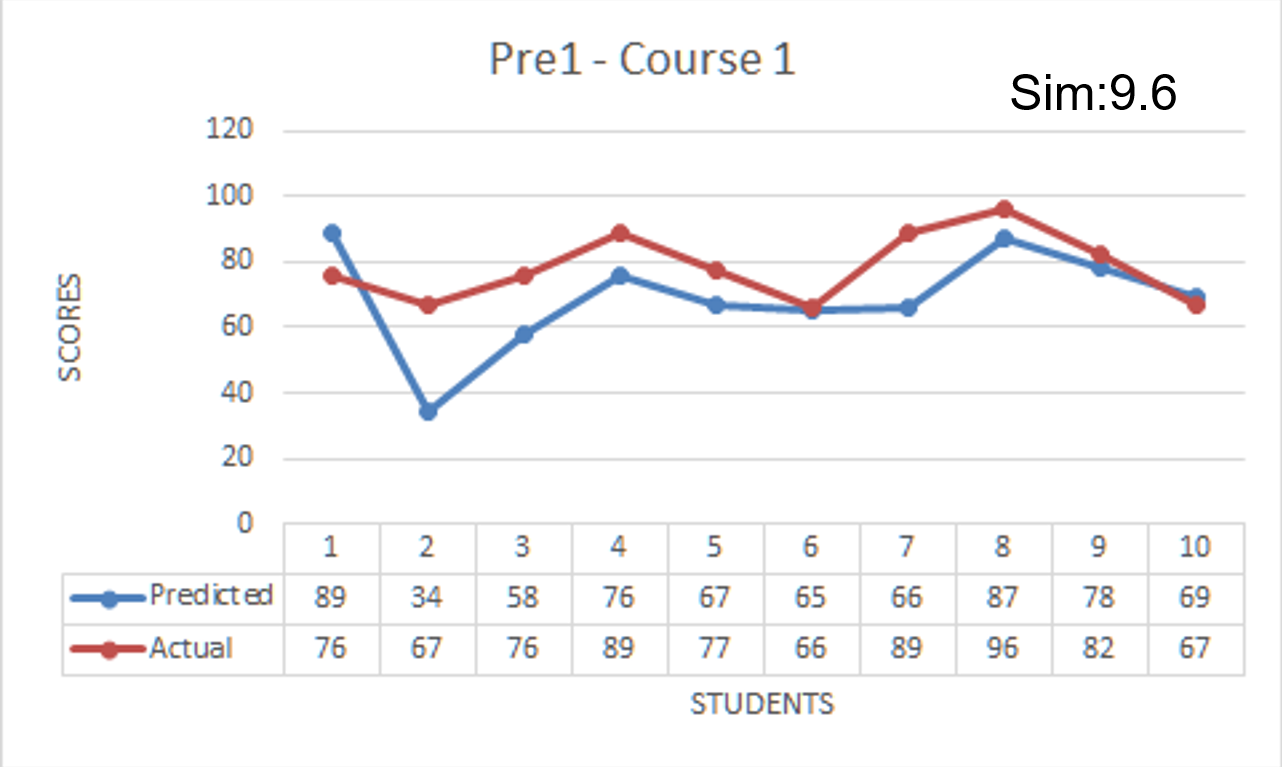
\includegraphics[width=\columnwidth]{figs/measure} 
	\caption{Our method based on item-based recommender system, Pre1 clearly benefit Course1 with a beachmark 9.6}
	\label{fig:sample}
\end{figure}

From Fig. 6, we can clearly see that most of the 10 students who have taken both Pre1 before Course1 have better actual scores than the prediction which is based on the overall performance. In other words, compared with the students whose overall performance is similar but without taking Pre1, these students have gotten 9.6 more points on Course1 averagely, which is a great improvment. Therefore we can say, Pre1 should benefit Course1 even without knowing the contents of both two courses.

This new measurement gives us a better way to measure the actual benefits a course may give to the other. In stead of using Pearsonal Corrleations, it is a more solid way because it can tolerate the influence of the students’ consisitent performance and also avoid the direct comparsion using scores of different courses. Using this method, we get a much better distribution of the overall benefits measurement. Specifically,  for the computer science department, there are 1191 pairs of courses have benefit benchmarks.The benefits points range from -17.9 to 12.6(Fig 7). Minus points mean the negative influence and positive points mean active influence. In the current version of our adjacency matrix , we ignore the negative points, which we also also color it as a difference color. This maybe one of our future work.
\begin{figure}[h]
	\centering % avoid the use of \begin{center}...\end{center} and use \centering instead (more compact)
	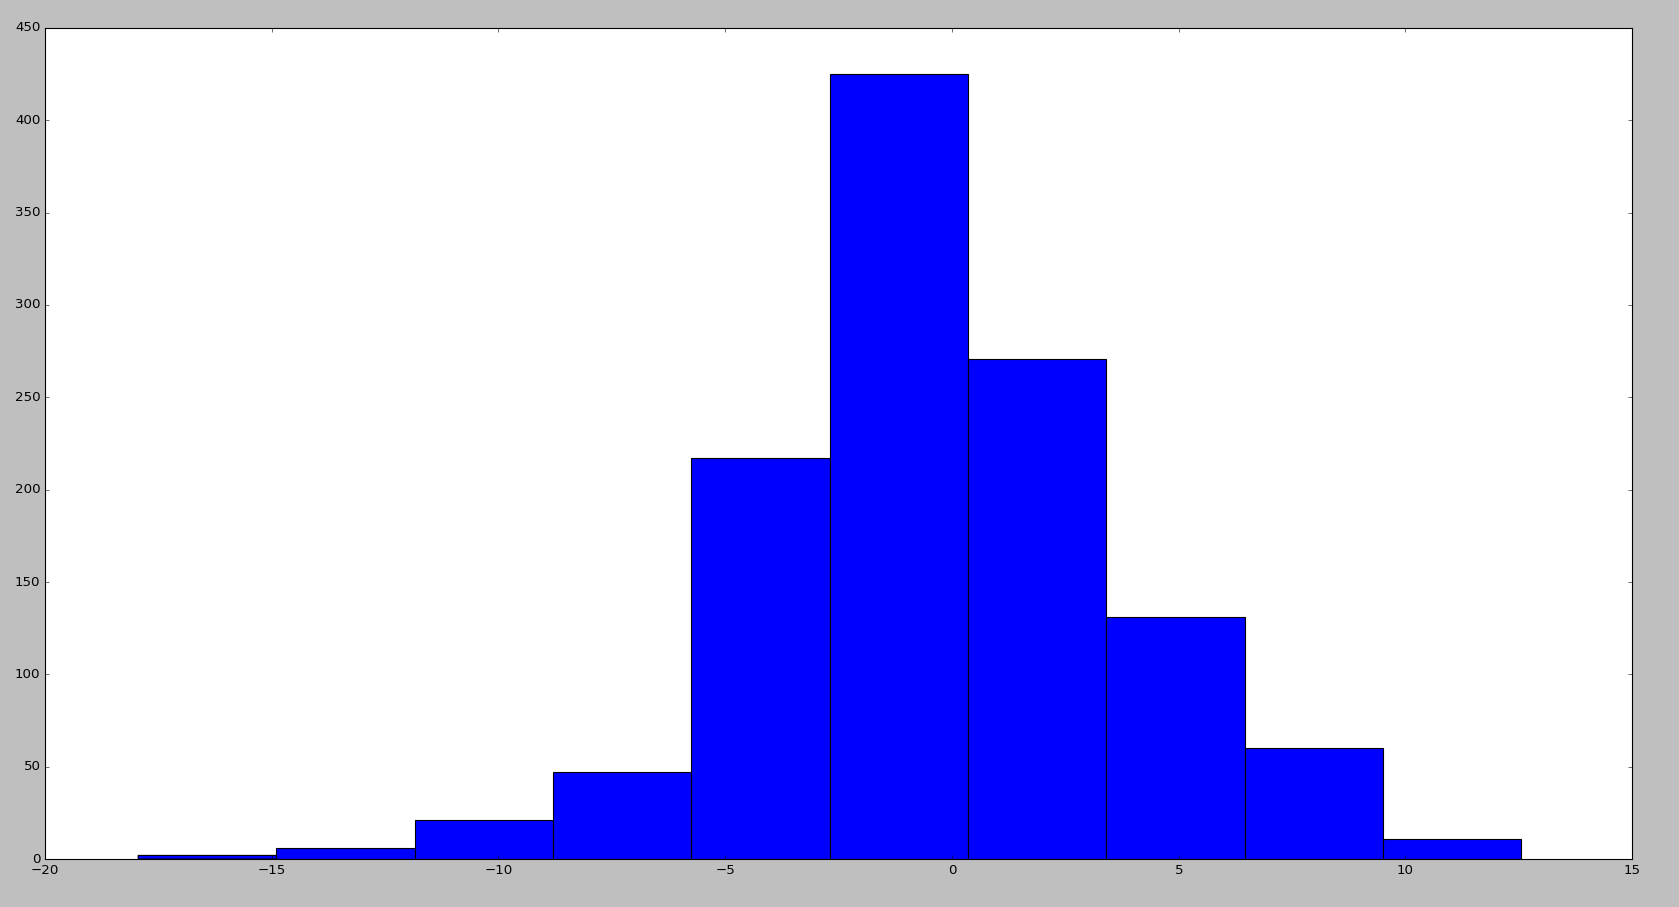
\includegraphics[width=\columnwidth]{figs/markdistribution} 
	\caption{The distribution of benefits benchmarks for CS courses, ranging from -17.9 to 12.6,bigger the number, more benefits may exit}
	\label{fig:sample}
\end{figure}

\subsection{Bar Chart View}
\label{sec:bar}
The bar chart view details the course users are interested in. The interaction is built between the adjacency matrix and the bar chart. When the user finds one course he is interested and wants to see all the courses may benefit this course. They can click on any grid along the column of that course. The bar chart will pop up. It reveal the top 10 courses which may benefits the selected course and order them by the benefit benchmarks. The color of each bar is the same as the corresponding grid in the adjacency matrix to make sure the consistency and.  This style avoid the possible confusion when users are navigating to the bar chart view. Using this bar chart view, users can easily find out for the specific course, which one has the highest benefit benchmark. Also, for a pair of courses, what’s the rank of the pre-course, is that actually a good choice? The view helps users to figure out these problems and make good decision for choosing good prerequisites. 
\begin{figure}[h]
	\centering % avoid the use of \begin{center}...\end{center} and use \centering instead (more compact)
	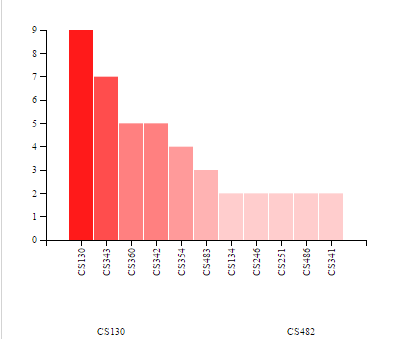
\includegraphics[width=\columnwidth]{figs/barchart} 
	\caption{Bar chart view for course CS482}
	\label{fig:sample}
\end{figure}

\subsection{Parallel Coordinates View}
\label{sec:parallel}
For a pair of courses we are interested in,  we use a parallel coordinates graph to show the specific grades changes for students who have taken both courses. Each line’s start point is the score that a student gets in the previous course, and the end point is the score the same students gets in the later course. The interaction is build between the adjacency matrix and the parallel coordinates. When a gird is clicked, a parallel coordinates will be shown in this view. Instead of focusing on the course level and getting a summarized benchmark  for each pair of courses. The parallel coordinates will allow users to explore the details and show all the trends of each student’s performance between theses two courses. Users can clearly observe the changes of each student which can be  a good reference when they are considering the benefit between two courses. For example ,from Fig. 9, the overall benefit CS240 may bring to CS492 is high positive. But we can also find some obvious outliners: a student getting almost 98 points gets 65 in the CS492, another student whose score for CS240 is 78 ends up getting 8 points in CS492. These are some anomalies which users can easily find out with the parallel coordinates. Fo r the future work, different colors are utilized to show the grade section for the course. And we also need to build  interaction between bar chart and parallel coordinates.
\begin{figure}[h]
	\centering % avoid the use of \begin{center}...\end{center} and use \centering instead (more compact)
	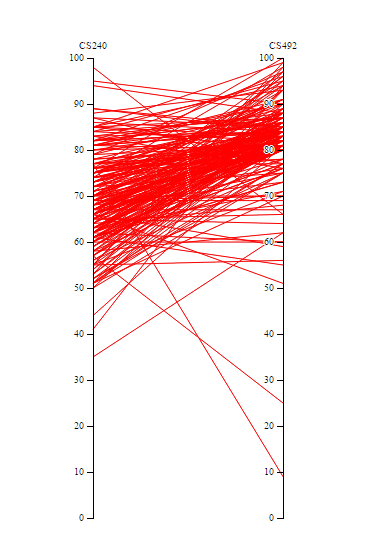
\includegraphics[width=\columnwidth]{figs/parallel} 
	\caption{Parallel coordinates graph for CS240-CS492}
	\label{fig:sample}
\end{figure}

%\begin{figure*}[h]
% \centering 
% 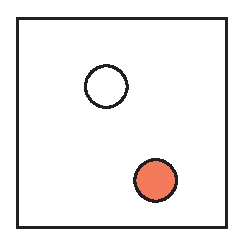
\includegraphics[width=\textwidth]{figs/sample} 
% \caption{Double Column Figure.}
% \label{fig:sample2}
%\end{figure*}



\section{Evaluation} % or "Research Plan"
\label{sec:vis}

In this section, we show some user studies and the results of your visualization. Since our data comes from a real world university, we can actually know the contents of each course and by consoling computer scientists, we can see if Coursim actually gives us some good perquisites for a chosen course. We also show our evaluation plan here for doing an actual user study.

\subsection{Usage Scenario}
\label{sec:usage}

This case study shows three different usages of this tool. First, when a student comes to his advisor and asked him a question like “what courses do I need to take this semester if I eventually want to take CS482?” The professor doesn’t know how much about CS482, actually the professor is just a Math Doctor which his student takes the CS as a minor. But using our tool, when can find the course CS482 in the adjacency matrix and click the column. Then in the bar chart ( Fig. 8), he can easily figure out that the CS130 and CS343 have the highest benchmarks. Then he moves to the matrix and clicks on the gird of pair CS130 –CS482 and CS343-CS482. The parallel oordinates tell him the most the students are enhanced if they have taken CS130 and CS343. With this knowledge in mind, he can advise the two courses to his students without knowing what actually the two courses are. What's more, another interesting question a student may be wondering is that if he has taken a course, which course he may take next which will be easiler for him to get a high score. For this purpose, he can find the row of that course, and go through the row and find out the red girds. Then he can click on it and see the details in the bar chart and parallel coordinates. The last example is that it can be used to evaluate the setting of  the current prerequisites. We can easily achieve that by finding out the pair of courses and watch its actual ranks in the barchart. Using the bar chart and parallel, a professor can figure out if the current prerequisites is a good. Are there any other hidden prerequisites which have a higher benefit than the current one? Or what’s actual performance looks like for students taking the prerequisites?

After plotting the pictures, we want to find out if the benchmarks work well. We pick up some pair of courses and find out the contents and titles of the university’s websites. The results shown are quite interesting. For example CS 365 and CS489, the benchmark we calculate is 11.2. CS365 is  Model of Computation and CS 489 is a topic course which includes Big Data Infrastructure, Complexity of Computational Problems and Introduction to Machine Learning, which include a lot of model computation.Some other pairs of courses with high benchmarks are also convinced by different domain specialists there are a lot of connections between these pairs. For instance, CS 135 Designing Functional Programs and CS 445: Software Requirements Specification and Analysis, CS 458: Computer Security and Privacy-CS 456 Computer Networks.


\subsection{Evaluation Plan}
\label{sec:plan}

As we stated in the original proposal, an intermediate evaluation test would be comparing documented dependency to the overview drawn by our tool. The overview should be a superset of documented dependency but not close to a universal set. We can worry less about false positives because the prototype doesn't have a high density of highlighted cells.

The above test can be automated relatively easily. We may not even need to get user involved. The ratio of identified documented dependency over all documented dependency should be the prime and only thing to look at in my opinion.

After that, an evaluation of false positives may be carried out. I see two possibilities: first is to contact the academical advisor from our dataset's university to confirm the possible dependency revealed by our tool; second is to find a local academical advisor who is willing to share her data and apply our tool to it. In fact, doing both would be more convincing.

Eventually, a user study should be done. We should have an academical advisor's feedback and improved the tool at this moment. We then ask the academical advisor to use this tool with students seeking advice, when they choose their courses. We need to be careful about the user groups here. Do we want to work with the same academical advisor all the time? Do we care about gender balance, student year(freshman, senior) balance?

I think we should share this tool with a handful of academical advisors, to avoid the tool being too personalized. When their feedback conflicts, we record their argument first and ask them if they are willing  to discuss further. We end up either solving the issue or having one implementation but understanding the alternatives. 

For a balanced student group, the question boils down to who's going to actually use this tool. If the tool is going to be used sololy with both student and academical advisor in presence, then we should accept whoever comes to the office and don't worry about balance at all. If the tool is going to be offered in the school system open to all students, we should invite students to evaluate it online in addition to academical office deployment. I'm more inclined to the first approach simply because it is easier to come true.

Existing tools should be considered in doing all these evaluations. A survey should be taken, asking users to rate all three views on a Likert scheme, with an optional text box of why they like or hate any part. Depending on the skewness, we maybe need to throw away the top 5\% high and low gradings. The text feedback should be synthesized to explain the gradings of each view and discussed possible improvement.


\section{Discussion}
\label{sec:discussion}

The project is successful overall. We learned valuable lessons throughout. They are about both general research and visualization research.
\begin{itemize}
\item Knowing what's out there in the field is important. Researchers at entry level often start out experimenting their own thoughts without studying literatures. Reference is more than citation. Readers will not be convinced unless we can relate other people's work to ours and explain why, how, and what we are doing differently.
\item During this project, we find it really helpful to summarize the problems of published papers. These problems serve as good reminders of common pitfalls even for experienced researchers and reviewers. We also think going back to the first slides at the beginning of semester to be useful. It helps keep the project going in a regular track.
\item For the coding part, d3 is a quite different language from C-style ones. We started out skimming preliminary tutorials and moved on to modify the gallery codes. This approach turned out to be inefficient and painful. I personally misunderstood chaining methods until mid term. If one happens to be familiar with C-style languages like me, d3 is likely to deserve more time to acquire than you anticipate.
\item Time management is crucial. It's dangerous to wait till last minute. We usually set for ourselves a dummy deadline, one or two days prior to the real deadline. We thus apply major fixes early and have enough time for minor fixes in a relaxed mood, which actually improves the quality of those minor fixes.
\end{itemize}



\paragraph*{Ongoing work}
\label{sec:conclusion}

Now let's review our tasks listed in Section 3. For task 1, we applied a NLP model and different kernel methods to summary the simulations as much as we can to get a overview quantitatively. For task 2, we build a context visualization to illustrate the details of the specific simulation. The design principle of this view is to remain the ground truth as much as possible. For task3, we follow the focus and context design, which allows user to spot the earthquake simulation they are interested and explore it in the context view. The prototype looks promising for now, since it provides a way to explore the whole earthquake dataset. In the meanwhile, there are  a lot of points for us to complete.

Even with the matrix diagram visualizations, the screen becomes cluttered as the number of simulation gets larger. In the future, when we get thousands of simulations, the matrix diagram will not scale. It is also worth considering if it's possible to cluster earthquakes hierarchically to maintain visual scalability. The way we choose periods for segmentation is also clearly inappropriate; we are currently investigating how to enable our machine learning methods with multiple overlapping motifs ([T3]).
Finally, even though we have worked with domain experts in developing these tools, a thorough validation of the designs, for example,   efficient navigation and interaction between different views, remains to be done.


%\bibliographystyle{abbrv}
\bibliographystyle{abbrv-doi-hyperref}
%%use following if all content of bibtex file should be shown
%\nocite{*}
\bibliography{report}
\end{document}

